%!TEX root = ../template.tex
%%%%%%%%%%%%%%%%%%%%%%%%%%%%%%%%%%%%%%%%%%%%%%%%%%%%%%%%%%%%%%%%%%%%
%% chapter5.tex
%% NOVA thesis document file
%%%%%%%%%%%%%%%%%%%%%%%%%%%%%%%%%%%%%%%%%%%%%%%%%%%%%%%%%%%%%%%%%%%%

\typeout{NT FILE chapter5.tex}%

\chapter{Plano de Trabalho}
\label{cha:work_plan}

\glsresetall
\prependtographicspath{{Chapters/Figures/Covers/}}

\section{Tarefas após a Discussão do Relatório}
\label{sec:tasks_after_discussion}

Essas tarefas visam consolidar a componente prática, reunir evidências
empíricas e garantir a redação final da dissertação. A seguir,
descrevem-se as atividades previstas:

\begin{itemize}
  
  \item \textbf{Desenvolvimento e Implementação}
  
  A fase de desenvolvimento consiste na concretização do protocolo em estudo
  de caso e/ou cenários simulados. Inclui a configuração de ambientes de
  teste, a execução de simulações que representem diferentes níveis de
  horizontalidade e a aplicação iterativa de contramedidas diante de
  cenários de ameaça. Os principais objetivos desta etapa são:
  \begin{itemize}
    \item \emph{Implementar} os elementos essenciais do protocolo, tais como
    mecanismos de consenso, sistemas de registro imutável e recursos de
    participação democrática.
    \item \emph{Testar} a eficácia, a eficiência e a resiliência do protocolo em
    situações com diferentes níveis de complexidade, incluindo possíveis
    cenários de falha ou de necessidade de centralização temporária.
    \item \emph{Recolher} dados empíricos (métricas de desempenho, logs de
    auditoria, feedback dos participantes) para sustentar a análise
    posterior.
  \end{itemize}
  \vspace{1em}
  
  \item \textbf{Redação Final da Dissertação}
  
  Uma vez consolidados os resultados do desenvolvimento, iniciam-se
  ajustes e revisões do texto da dissertação, incorporando as
  evidências empíricas. Esta tarefa engloba:
  \begin{itemize}
    \item \emph{Integração} dos dados empíricos obtidos na fase anterior,
    apresentando resultados quantitativos e qualitativos que confirmem (ou
    refutem) as hipóteses de investigação.
    \item \emph{Discussão Crítica} das limitações do estudo, recomendações
    práticas e possíveis adaptações do protocolo para outros cenários.
    \item \emph{Revisão do Documento} de acordo com as diretrizes formais do
    programa e com eventuais sugestões oriundas do orientador ou do corpo
    avaliador.
  \end{itemize}
  \vspace{1em}
  
\end{itemize}




\section{Gantt Chart}
\label{sec:gantt_chart}


\begin{figure}[htbp]
  \centering
  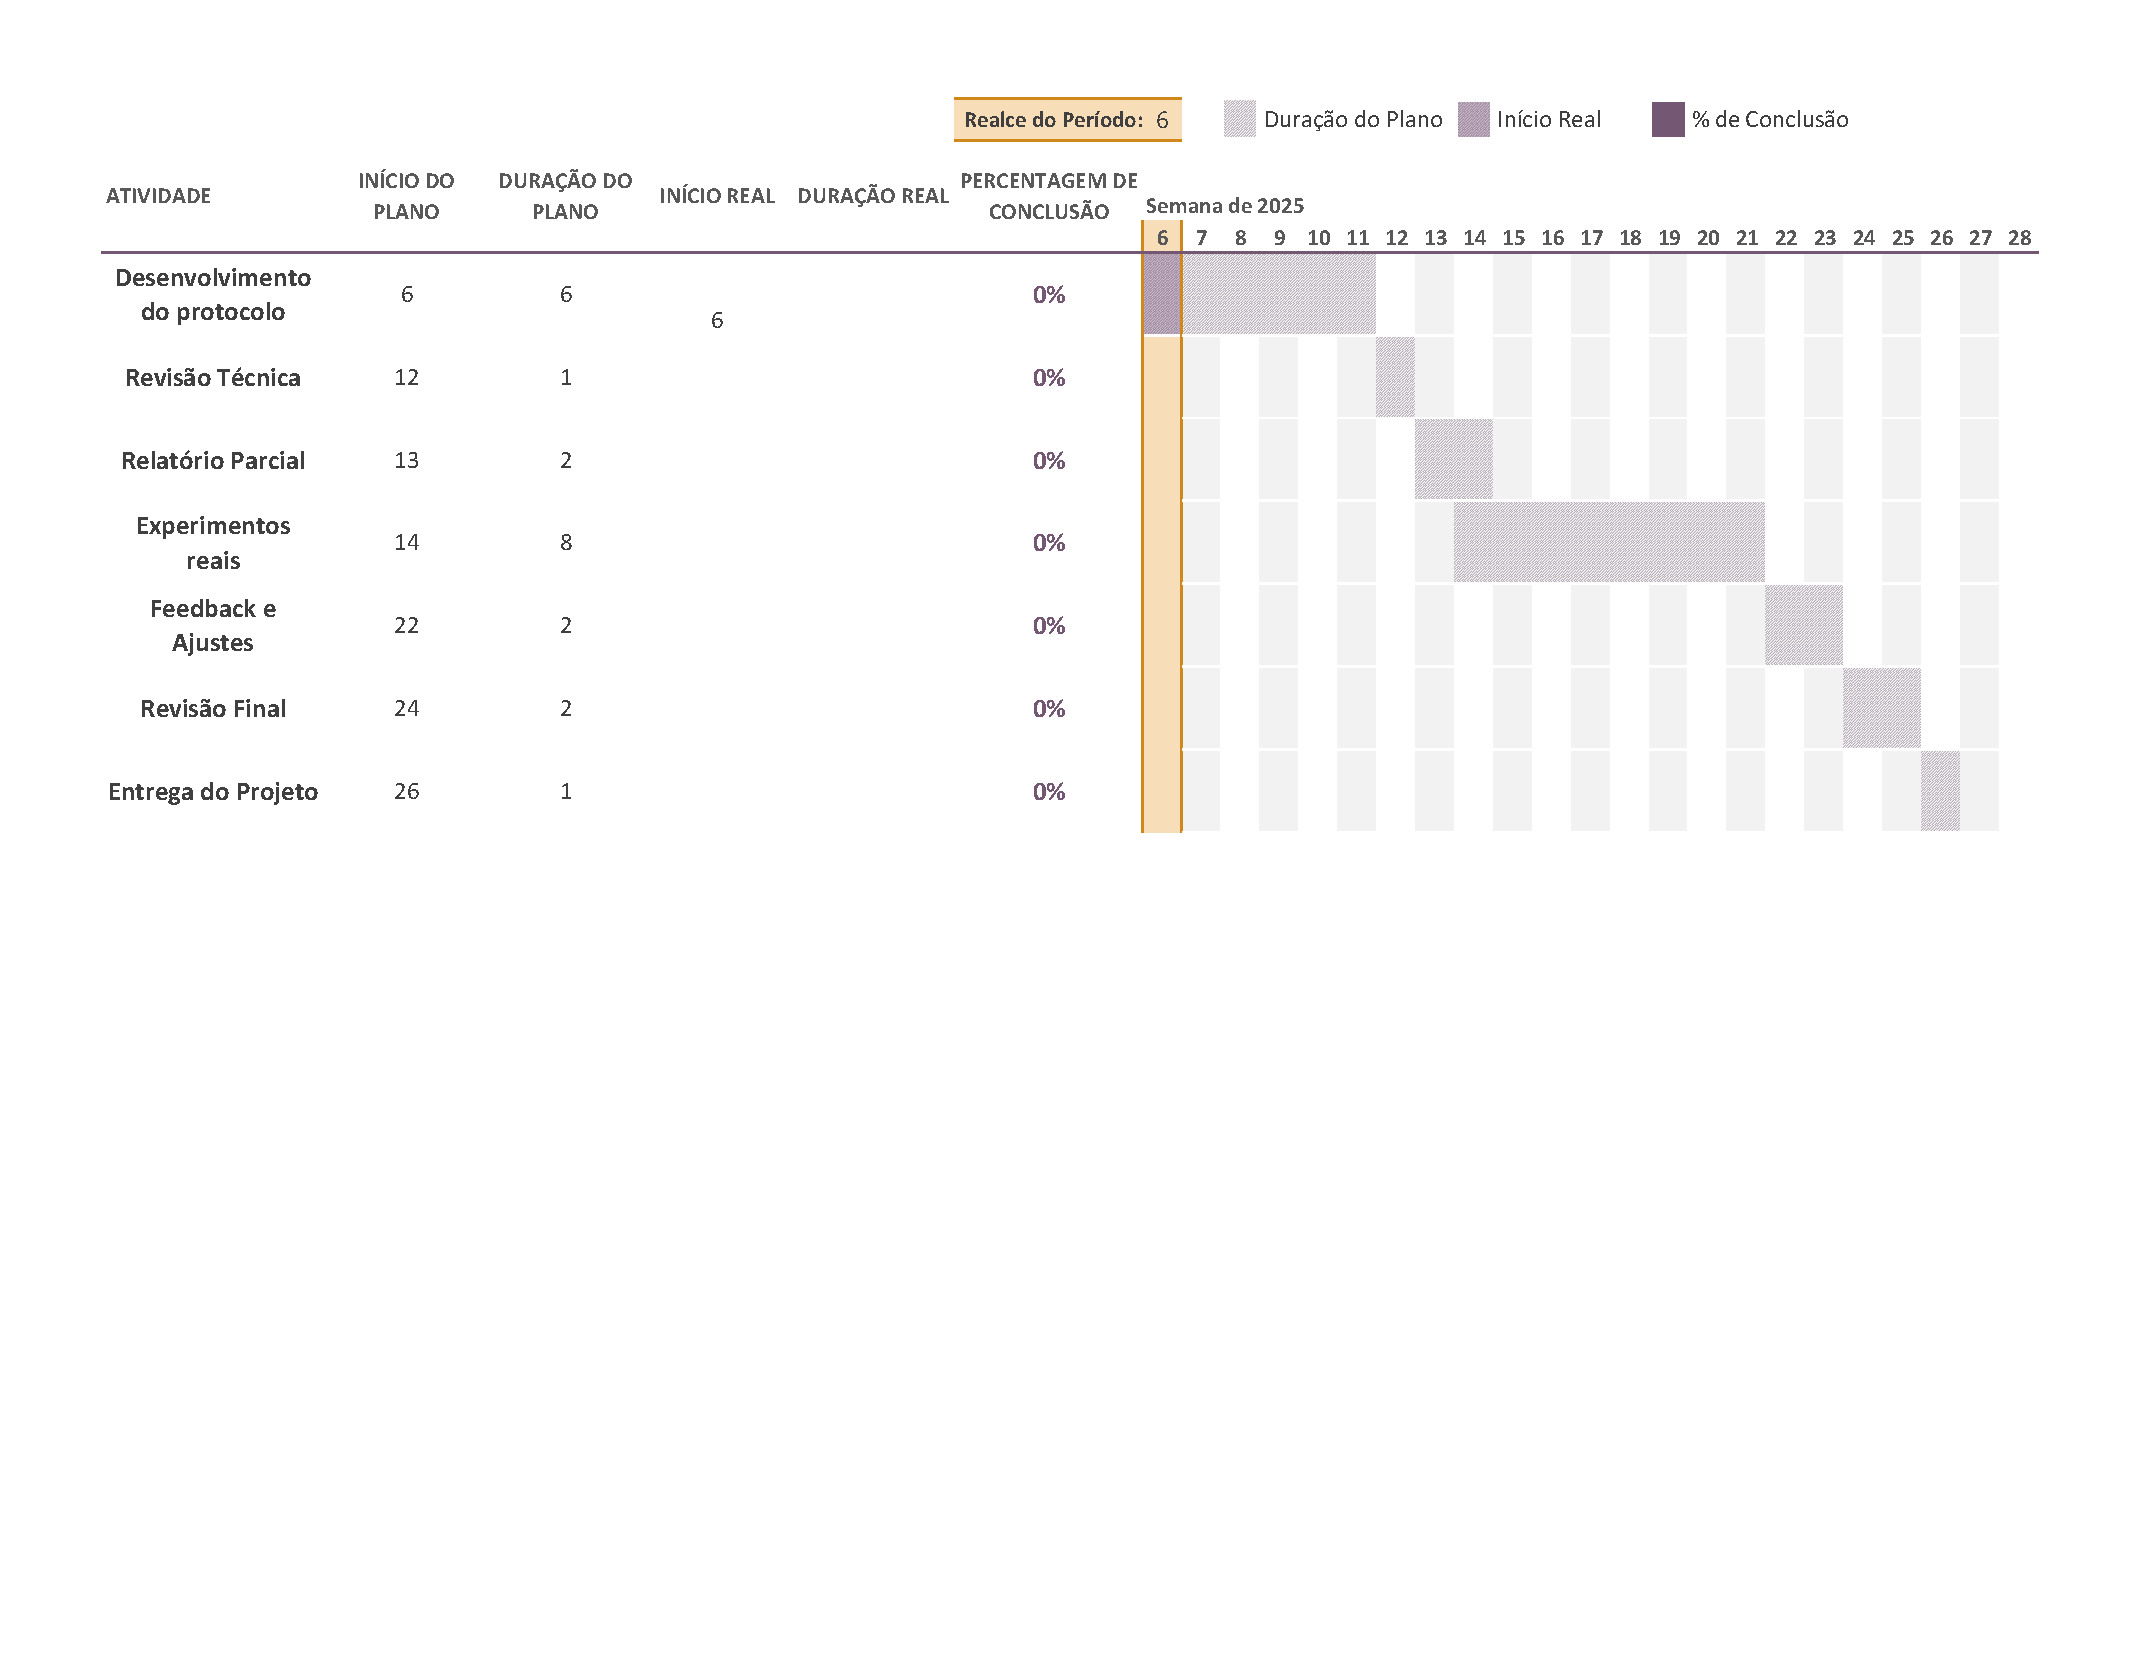
\includegraphics[width=1\linewidth]{Gantt}
  \caption{Gannt Chart.}
  \label{fig:Gannt}
\end{figure}